\documentclass[12pt, a4paper]{article}

\usepackage[hmargin=2.5cm, vmargin=2cm]{geometry}
\usepackage{amsthm, amssymb, mathtools, yhmath, graphicx}
\usepackage{fontspec, type1cm, titlesec, titling, fancyhdr, tabularx}
\usepackage{color}
\usepackage{unicode-math}
\usepackage{float}
\usepackage{hhline}
\usepackage{comment}
\usepackage[abbreviations]{siunitx}
\usepackage{csvsimple}
\usepackage{subcaption}
\usepackage{cleveref}
\usepackage{listings}
\definecolor{mygreen}{rgb}{0,0.6,0}
\lstset{
  basicstyle=\footnotesize\ttfamily,
  breaklines=true,
  keywordstyle=\color{blue},
  numbers=left,
  numberstyle=\tiny\color{mygray},
  commentstyle=\color{mygreen}, 
}

\usepackage[CheckSingle, CJKmath]{xeCJK}
\usepackage{CJKulem}
\usepackage{enumitem}
\usepackage{tikz}
\usepackage[siunitx]{circuitikz}
\usepackage{wrapfig}
\usepackage{sourcecodepro}
%\setCJKmainfont[BoldFont=cwTex Q Hei]{cwTex Q Ming}
%\setCJKsansfont[BoldFont=cwTex Q Hei]{cwTex Q Ming}
%\setCJKmonofont[BoldFont=cwTex Q Hei]{cwTex Q Ming}
\setCJKmainfont[BoldFont=cwTeX Q Hei]{cwTeX Q Ming}
\setmonofont{Source Code Pro}

\def\normalsize{\fontsize{12}{18}\selectfont}
\def\large{\fontsize{14}{21}\selectfont}
\def\Large{\fontsize{16}{24}\selectfont}
\def\LARGE{\fontsize{18}{27}\selectfont}
\def\huge{\fontsize{20}{30}\selectfont}

\newtheorem{lemma}{Lemma}

%\titleformat{\section}{\bf\Large}{\arabic{section}}{24pt}{}
%\titleformat{\subsection}{\large}{\arabic{subsection}.}{12pt}{}
%\titlespacing*{\subsection}{0pt}{0pt}{1.5ex}

\parindent=24pt

\DeclarePairedDelimiter{\abs}{\lvert}{\rvert}
\DeclarePairedDelimiter{\norm}{\lVert}{\rVert}
\DeclarePairedDelimiter{\inpd}{\langle}{\rangle}
\DeclarePairedDelimiter{\ceil}{\lceil}{\rceil}
\DeclarePairedDelimiter{\floor}{\lfloor}{\rfloor}

\newcommand{\unit}[1]{\:(\text{#1})}
\newcommand{\df}[1]{\mathop{}\!\mathrm{d^#1}}
\newcommand{\img}{\mathrm{i}}
\newcommand{\dD}{\mathrm{d}}
\newcommand{\dI}{\,\mathrm{d}}

\title{ \bf {\Huge Signal and System}\\ MATLAB Homework \#3}
\author{B02901178 江誠敏}

\begin{document}

\maketitle

\section{Problem 1}
\begin{enumerate}[label=(\alph*)]
  \item {\bf Find the inverse z-transform of (2). Please state the ROC. } \\[12pt]
    By using \texttt{residuez} command in Octave, we obtain
    \begin{multline*}
      H(z) \approx \frac{ 0.00682 + 0.40930 \img }{ 1 - (0.35750 - 0.58890\img) z^{-1} }
      + \frac{ 0.00682 - 0.40930\img }{ 1 - (0.35750 + 0.58890\img) z^{-1} } \\
      + \frac{ -0.10445 - 0.15963\img }{ 1 - (0.76860 - 0.33380\img) z^{-1} }
      + \frac{ -0.10445 + 0.15963\img }{ 1 - (0.76860 + 0.33380\img) z^{-1} }
      + 0.29287
    \end{multline*}

    so
    \begin{multline*}
      \mathcal{Z}^{-1} \{ H(z) \} =  (0.00682 + 0.40930 \img) (0.35750 - 0.58890\img)^n  \\
      + (0.00682 - 0.40930 \img) (0.35750 + 0.58890\img)^n  \\
      + (-0.10445 - 0.15963 \img) (0.76860 + 0.33380\img)^n  \\
      + (-0.10445 + 0.15963 \img) (0.76860 - 0.33380\img)^n  + 0.29287 \delta[n]
      \end{multline*}
    The maximum absolute value of the poles is about $0.83795$.
    Since the system is causal,  the ROC is $ \abs{z} > 0.83795 $
    \clearpage
  \item {\bf Find and plot the locations of poles and zeros.} \\[12pt]

    \begin{figure}[H]
      \centering
      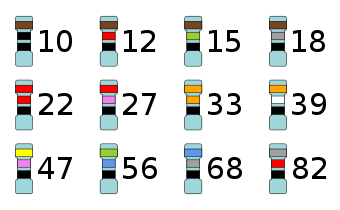
\includegraphics[width=0.7\textwidth]{fig1.eps}
      \caption{Plot of the poles and zeros.}
    \end{figure}


  \item {\bf Evaluate and plot the magnitude and phase response.} \\[12pt]
    The frequency response is simply $H(e^{\img \omega})$.
    Use \texttt{freqz} to plot the frequency response.
    \begin{figure}[H]
      \centering
      \begin{subfigure}{0.49\textwidth}
        \includegraphics[width=\textwidth]{fig2-1.eps}
        \caption{Magnitude response}
      \end{subfigure} %
      \begin{subfigure}{0.49\textwidth}
        \includegraphics[width=\textwidth]{fig2-2.eps}
        \caption{Phase response}
      \end{subfigure}
      \caption{Frequency response.}
    \end{figure}

    \clearpage

  \item {\bf Find a representation of this transfer function as a cascade of two second-order
    sections with real coefficients.} \\[12pt]
    By using the \texttt{zp2sos} command, we obtain
    \begin{align*}
      H(z) &= 0.0976 \left(\frac{ 1 + 2z^{-1} + 1z^{-2} }{ 1 - 0.71500z^{-1} + 0.47461z^{-2} }\right)
      \left(\frac{ 1 - 2z^{-1} + 1z^{-2} }{ 1 -1.53720 z^{-1} + 0.70217 z^{-2} } \right) \\
      &= 0.0976 H_1(z) H_2(z)
    \end{align*}

  \item {\bf Evaluate and plot the magnitude response of each section in 4.}\\[12pt]
    Their magnitude response is simply $H_1(e^{\img \omega}) \text{ and } H_2(e^{\img \omega})$

    \begin{figure}[H]
      \centering
      \begin{subfigure}{0.49\textwidth}
        \includegraphics[width=\textwidth]{fig3.eps}
        \caption{Magnitude response of $H_1$}
      \end{subfigure} %
      \begin{subfigure}{0.49\textwidth}
        \includegraphics[width=\textwidth]{fig4.eps}
        \caption{Magnitude response of $H_2$}
      \end{subfigure}
    \end{figure}

  \item {\bf Determine the impulse response of the system by obtaining the output for an input
    $x[n] = \delta[n]$ and compare it with the result of 1.}\\[-10pt]
    \begin{figure}[H]
      \centering
      \includegraphics[width=0.65\textwidth]{fig5.eps}
      \caption{Impulse response of $H$}
    \end{figure}
    They are identical.
\end{enumerate}

\end{document}

